\section{Background and Motivation}
Begin the introduction to your research topic here. Provide a brief background, define the context, and highlight the motivation for the study.

An example of a linear regression model is given by:
\begin{equation}\label{eq1}
  \bm{y = X\beta + \epsilon}
\end{equation}
where $\bm{y}$ is an $n \times 1$ vector of observations on the dependent variable, $\bm{X}$ is an $n \times p$ matrix of observations on the explanatory variables, $\bm{\beta}$ is a $p \times 1$ vector of unknown coefficients, and $\bm{\epsilon}$ is an $n \times 1$ vector of random error terms.

Equation~\ref{eq1} represents the standard linear regression model. The \gls{olse} is used to estimate the parameters of this model.

\section{Illustrative Examples}
\subsection{Example Figure}

Figure~\ref{fig1} presents a sample diagram to illustrate estimation.

\begin{figure}[!ht]
    \centering
    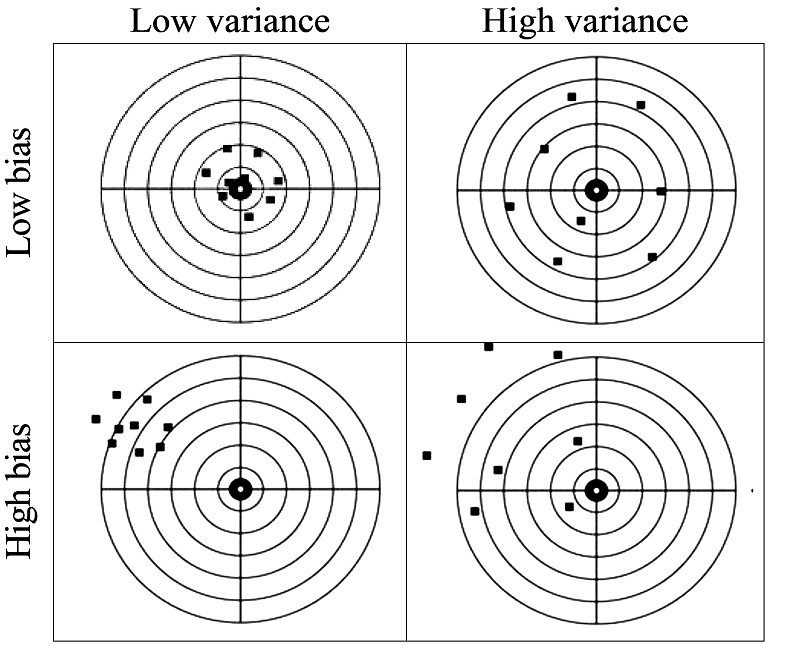
\includegraphics[width=3.5in]{bv.png}
    \caption{Illustration of parameter estimates and true values}
    \label{fig1}
\end{figure}

In Figure~\ref{fig1}, the central part indicates the actual values of the population parameter vector $\bm{\beta}$, while the dots represent the estimated values of $\bm{\beta}$. Ideally, both the bias and variance of these estimators should be minimal.

\subsection{Example Table}

Table~\ref{t1} demonstrates a sample data structure used in the study.

\begin{table}[H]
    \centering
    \caption{Example Table with Placeholder Values}
    \begin{tabular}{ccc} \hline
        \textbf{Col1} & \textbf{Col2} & \textbf{Col3} \\ \hline
        01 &  &  \\
        02 &  &  \\ \hline         
    \end{tabular}
    \label{t1}
\end{table}

Table~\ref{t1} consists of three columns and two rows. Actual data should be inserted here relevant to your study.

\section{Objectives of the Research}
Clearly state the main objectives of the research. These should align with the identified problem and research questions. For example:

\begin{itemize}
    \item To develop a statistical model for ...
    \item To analyze the impact of ...
    \item To evaluate the performance of ...
\end{itemize}

\section{Sample References}
Cite relevant literature using BibTeX or manual citations. Examples include:

- Journal article: \cite{Si86}
- Book: \cite{ro95}
- Thesis: \cite{Het16}
- Technical report: \cite{Te80}
